\documentclass[10pt,a4paper]{article}
\usepackage[utf8]{inputenc}
\usepackage{url}
\usepackage{amsmath}
\usepackage{amsfonts}
\usepackage{amssymb}
\usepackage{listings}
\usepackage{graphicx}

\usepackage{color}

\def\File#1{\textsf{#1}}
\def\Code#1{\texttt{#1}}
\def\Key#1{\textsf{#1}}

\definecolor{mygreen}{rgb}{0,0.6,0}
\definecolor{mygray}{rgb}{0.5,0.5,0.5}
\definecolor{mymauve}{rgb}{0.58,0,0.82}

\lstset{ %
  backgroundcolor=\color{white},   % choose the background color; you must add \usepackage{color} or \usepackage{xcolor}
  basicstyle=\footnotesize,        % the size of the fonts that are used for the code
  breakatwhitespace=false,         % sets if automatic breaks should only happen at whitespace
  breaklines=true,                 % sets automatic line breaking
  captionpos=b,                    % sets the caption-position to bottom
  commentstyle=\color{mygreen},    % comment style
  deletekeywords={...},            % if you want to delete keywords from the given language
  escapeinside={\%*}{*)},          % if you want to add LaTeX within your code
  extendedchars=true,              % lets you use non-ASCII characters; for 8-bits encodings only, does not work with UTF-8
  frame=single,                    % adds a frame around the code
  keywordstyle=\color{blue},       % keyword style
  language=Octave,                 % the language of the code
  morekeywords={*,...},            % if you want to add more keywords to the set
  numbers=left,                    % where to put the line-numbers; possible values are (none, left, right)
  numbersep=5pt,                   % how far the line-numbers are from the code
  numberstyle=\tiny\color{mygray}, % the style that is used for the line-numbers
  rulecolor=\color{mygray},         % if not set, the frame-color may be changed on line-breaks within not-black text (e.g. comments (green here))
  showspaces=false,                % show spaces everywhere adding particular underscores; it overrides 'showstringspaces'
  showstringspaces=false,          % underline spaces within strings only
  showtabs=false,                  % show tabs within strings adding particular underscores
  stepnumber=2,                    % the step between two line-numbers. If it's 1, each line will be numbered
  stringstyle=\color{mymauve},     % string literal style
  tabsize=2                       % sets default tabsize to 2 spaces
%  title=\lstname                   % show the filename of files included with \lstinputlisting; also try caption instead of title
}

\title{01435 Practical Cryptanalysis\\Project 3}
\author{Kim Rostgaard Christensen - s084283}
\begin{document}
\maketitle
\begin{abstract}
The purpose of this report is to document the tool developed for decrypting cipher-text and recovering keys generated with the Linear Congruence Generator from GCC (old glibc).\\
Full sources can be found at:\\
 \url{https://github.com/rostgaard/practical_cryptoanalysis/}
\end{abstract}

\section*{Project description}
A file with ciphertext, a description of the key generation, and an approximate date of key generation, which is used as seed, is given.\\
The purpose is then to implement a tool that decrypts ciphertext.

\section*{Design and implementation}
The first step of the tool will be to generate the keys needed for decrypting. Validation can be done by detecting non-printable characters. For speed purposes, only the first 16 bytes will be decrypted in the evaluation step.\\
For the implementation the package \Code{Ada.Streams.Stream\_IO} was used to read in files. This enables us to treat a file as a stream - enabling us to read raw bytes without being affected by control signals. In this tool, the entire buffer is read to memory - but could just as easily be streamed in chunks.\\
Every key is generated in a hashed map, so we can ensure uniqueness of the keys. At the end  of key generation, every key is checked using the non-printable-characters-check.
\section*{Usage}
The tool is command-line only, and take at least one parameter; the path to the ciphertext tile.\\
You can also give the tool an additional argument which is the maximum keys it should try to find. For this case, 256 is enough, and we can quit early. Giving no arguments will result in a ``usage'' description printed to the command line.

\section*{Observations}
During development, one thing became apparent: There were only 256 distinct keys.\\
Investigating further, we found that every byte value occurred exactly 16 times, and once in every index. Diving the keys into two halves and plotting them, gives the pattern shown in figure \ref{fig:scatter_plot}.
\begin{figure}[h]
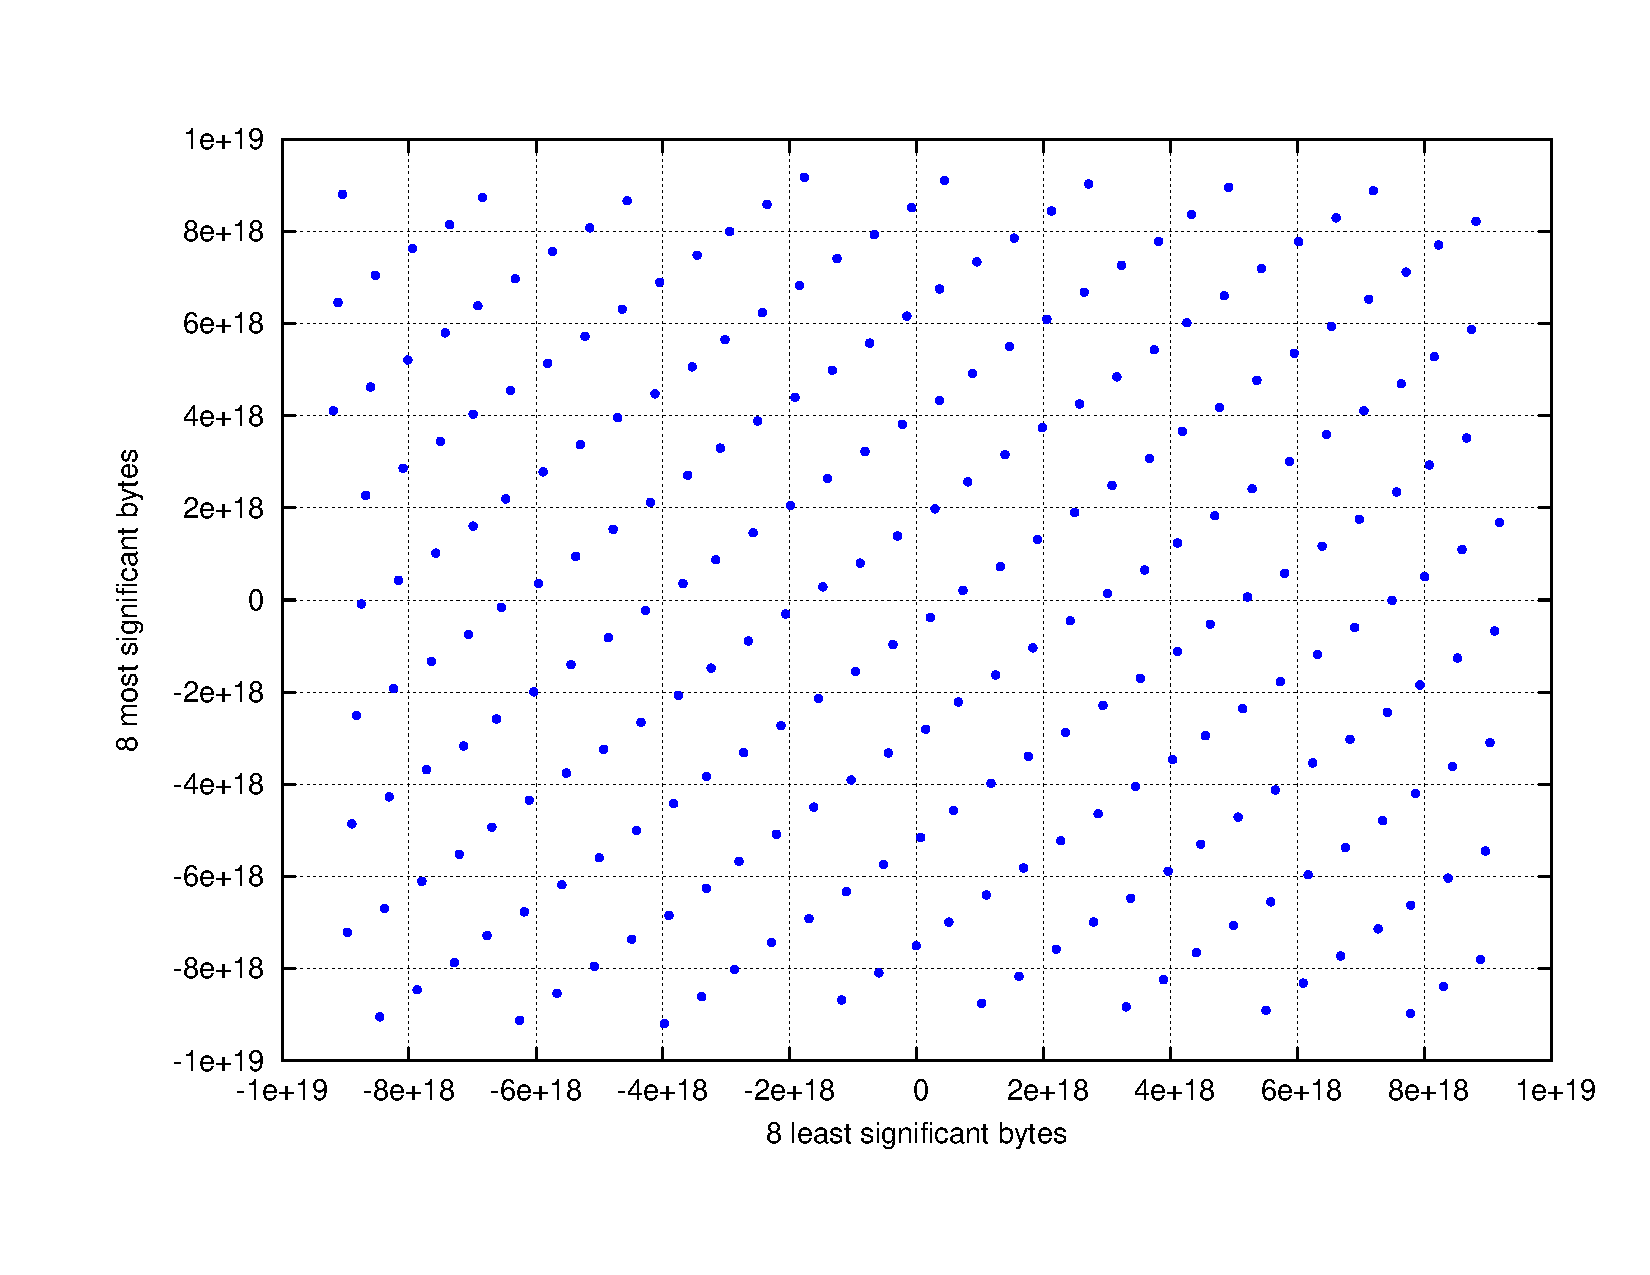
\includegraphics[scale=0.45]{../output/scatter.pdf}
\caption{MSB/LSB plot}
\label{fig:scatter_plot}
\end{figure}


\section*{Further work}
If the keyspace is large, it may be infeasible to save all unique keys prior to trying them. Instead of trying all keys, a large LRU\footnote{Least Recently Used} buffer could hold the latest tried ones.
\end{document}